

\subtitle{Linear Combination and Matrix Multiplication}\maketitle
\aaa{Learning Objectives}
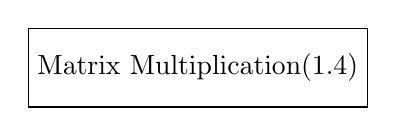
\begin{tikzpicture}[transform shape, block/.style={draw, rectangle, minimum width=2cm, minimum height=1cm}]
\node[block] (block1) {Matrix Multiplication(1.4)};
\end{tikzpicture}

\begin{itemize}
\item How to multiply two matrices?
\begin{itemize}
	\item what size of matrices can be multiply.
\end{itemize}
\item How to represent a matrix by math symbol?
\item Matrix multiplication through linear combination of columns
\item Matrix multiplication through linear combination of rows 
\item Doing algebra with matrices
\begin{itemize}
\item Is $AB=BA$?
\item How to expand $(A+B)(A-B)$ or $(A+B)^2$ ?
\end{itemize}
\item Some special matrices
\begin{itemize}
\item Upper triangular, lower triangular matrices.
\item Diagonal matrices, symmetric matrices.
\end{itemize}
\end{itemize}

\x{Explain matrix multiplication to elementary school students!}


\a{Matrix Multiplication}
%\apple\peach\bean\soup\lemon\leaf\milk\coffee\carrot\cola\tea\cow\orange

%\a\aa
Shinchan is operating a coffee shop, making various drinks. For each drink he need the following ingradients.
$$
\begin{cases}
\text{Milk }\milk: \text{ need } \cow;\\
\text{Lemon Tea}\tea:\text{ need } \leaf \leaf \lemon;\\
\text{Coffee}\coffee:\text{ need } \bean \bean\\
\end{cases}
$$
\a\aa
To make it clear, he made it into a table
\[columns]{
\column{0.6\textwidth}
$$
\t{}\milk\coffee\tea,\leaf002,\lemon001,\bean020,\cow100.
$$
\column{0.4\textwidth}
\hi
}
%$$
%\t{}\leaf\lemon\bean\cow,\milk0001,\coffee0020,\tea2100.
%$$\rightline\hi
\a\aa

People like those drinks, to sale it better, Shinchan designed the following meal plan
$$
\t{}\bento\soup,
\milk21,
\coffee02,
\tea11.
$$
$$
\begin{cases}
	\text{Meal 1}\bento: \text{2 milks and 1 tea} ;\\
\text{Meal 2}\soup:\text{1 milk 2 coffee and 1 tea};\\
\end{cases}
$$
Let us call \bento,\soup \x{compunds} and \milk,\tea\coffee \x{materials}.
\a\aa
To prepare for each meal, Shinchan need to know how much material is needed, can you combine those two table for him?

\[columns]{
\co{37}\t{}\milk\coffee\tea,\leaf002,\lemon001,\bean020,\cow100.
\co{28}\t{}\bento\soup,
\milk21,
\coffee02,
\tea11.
\co3
\t{}\bento\soup,\leaf{}{},\lemon{}{},\bean{}{},\cow{}{}.
}
\a\aa
Mathematically, we call the table of the ingradients to produce something as the \alert{matrix}. The combination of two ingradients is called the \alert{matrix multiplication}.  

\[equation]{\label{equation:multiplication}\overbrace{\t{}\milk\coffee\tea,\leaf{0}{0}{2},\lemon{0}{0}{1},\bean{0}{2}{0},\cow{1}{0}{0}.}^{\text{left factor}}\overbrace{\t{}\bento\soup,
\milk{2}{1},
\coffee{0}{2},
\tea{1}{1}.}^{\text{right factor}}\quad=
\overbrace{\t{}\bento\soup,\leaf{2}2,\lemon{\alert1}{\alert1},\bean{0}4,\cow{2}1.}^{\text{product}}}

\a{Matrix notation}
For the product
$$
\t{}\milk\coffee\tea,\leaf{0}{0}{2},\lemon{0}{0}{1},\bean{0}{2}{0},\cow{1}{0}{0}.\t{}\bento\soup,
\milk{2}{1},
\coffee{0}{2},
\tea{1}{1}.=
\t{}\bento\soup,\leaf{2}2,\lemon{\alert1}{\alert1},\bean{0}4,\cow{2}1.
$$
mathematically we write 
$$
\m002,001,020,100.\m21,02,11. = \m22,11,04,21.
$$

\a\aa
When representing matrices abstractly, the subindices are arranged 
$$
a_{\text{row number, column number}}
$$
and whenever one write $A= (a_{ij})$, he means
$$
A=\m 
{a_{11}}{a_{12}}{\cdots}{a_{1n}},
{a_{21}}{a_{22}}{\cdots}{a_{2n}},
\vdots\vdots\ddots\vdots,
{a_{m1}}{a_{m2}}{\cdots}{a_{mn}}.
$$
\vfill
\textbf{Exercise:}
If 
$$
A = (a_{ij}) = \m 12,34.
$$
Write down the value of $a_{11}$, $a_{12}$, $a_{21}$ and $a_{22}$.



\a{Size of a matrix}

\[defi]{If a matrix $A$ has $m$ rows and $n$ columns, we say that $A$ is an $ m \times n $ matrix.}
We see that if $A$ is $m \times n$ matrix, 
\begin{enumerate}
\item $m$ = number of rows = number of \x{materials}
\item $n$ = number of columns = number of \x{compunds}
\end{enumerate}
\a\aa
There are only 3 material lists playing the role in $C=AB$. Put
\begin{enumerate}
\item $m=$ Number of materials of $A$;
\item $n=$ Number of compunds of $A = $ Number of materials of $B$;
\item $p=$ Number of compunds of $B$ ;
\item Materials of $A$ = Matrials of $C$
\item Compunds of $B$ = Compunds of $C$
\end{enumerate}
$$
\overbrace{\t{}\milk\coffee\tea,\leaf{0}{0}{2},\lemon{0}{0}{1},\bean{0}{2}{0},\cow{1}{0}{0}.}^{A}\overbrace{\t{}\bento\soup,
\milk{2}{1},
\coffee{0}{2},
\tea{1}{1}.}^{B}=\overbrace{\t{}\bento\soup,\leaf{2}2,\lemon{\alert1}{\alert1},\bean{0}4,\cow{2}1.}^{C}
$$



\a\aa
\[prop]{The matrix multiplication $ AB $ makes sense only when 

\centerline{the number of \x{columns} in $ A $  $=$ the number of \x{rows} in $ B $}
The size is given by
$$
\underbrace{A}_{m\times n}\underbrace{B}_{n\times p} = \underbrace{C}_{m\times p}
$$
	}

\a\aa

\textbf{Exercise}: Without knowing entries. Let 
$$
A=\m ??,??,??.\qquad
B=\m ???,???,???,???.
$$
Which product is definable? $AB$ or $BA$?

\a\aa

Next we will study matrix multiplications from the perspective of \alert{entries}, \alert{columns} and \alert{rows}. You will see its relation with linear combination.

\a{Dot Product of rows and columns}
Each \alert{entry} of the ingradients corresponds to how much the material is needed for a single good.

$$
\t{}\bento\soup,\leaf{2}2,\lemon{1}{\h1},\bean{0}4,\cow{2}1.
$$

\soup need 1 \lemon.
\a\aa
To know how many \lemon is needed for \soup. Notice that \soup are made of \alert{semi-finished meals} \milk,\coffee and \tea. It is sufficient to know how many \lemon is needed by those semi-finished meals.
\[columns]{
\co{5}\t{}\milk\coffee\tea,\leaf{0}{0}{2},\lemon{\h0}{\y0}{\e1},\bean{0}{2}{0},\cow{1}{0}{0}.
\co{5}\t{}\bento\soup,
\milk{2}{\h1},
\coffee{0}{\y2},
\tea{1}{\e1}.
}

\aaa


\aaa{Product by entries}
\a\aa
We represents the need by the following graph


\[z]{
\node (A) at (0, 0) {\soup};
\node (B) at (-4, -2) {\t{\h1\milk}.};
\node (C) at (0, -2) {\t{\y2\coffee}.};
\node (D) at (4, -2) {\t{\e1\tea}.};
\node (E) at (-4, -4) {\t{\h1\milk\text{needs}$1\times 0$\lemon}.};
\node (F) at (0, -4) {\t{\y2\coffee\text{needs}$2\times 0$\lemon}.};
\node (G) at (4, -4) {\color{white}\t{\e1\tea\text{needs}$1\times 1$\lemon}.};
\node (H) at (0, -6) {\lemon};
\node (I) at (0,-7) {Total demand: $\t{\h1}.\times \t{\h0}.+\t{\y2}.\times \t{\y0}.+\t{\e1}.\times \t{\e1}.=1$};

% arrows
\draw[<-,ultra thick%, to path={-| (\tikztotarget)}
]
  (A) edge (B)  edge (C) edge (D) (B) edge (E) (C) edge (F) (D) edge (G);
\draw[->,ultra thick]
  (H) edge (E) edge (F) edge (G);
}
\aaa





\aaa{Product by entries}
\[prop]{In the matrix product $C=AB$. \alert{Each entry of C } is given by the corresponding inner product of a row of $A$ and a column of $B$}
\[columns]{
\co{35}$\overbrace{\t{}\milk\coffee\tea,\leaf{0}{0}{2},\lemon{\h0}{\y0}{\e1},\bean{0}{2}{0},\cow{1}{0}{0}.}^{A}$
\co{35}$\overbrace{\t{}\bento\soup,
\milk{2}{\h1},
\coffee{0}{\y2},
\tea{1}{\e1}.}^{B}\quad$=
\co{3}$\overbrace{\t{}\bento\soup,\leaf{2}2,\lemon{1}{\alert1},\bean{0}4,\cow{2}1.}^{C}$
}

$$1=\t{\h1}.\times \t{\h0}.+\t{\y2}.\times \t{\y0}.+\t{\e1}.\times \t{\e1}.$$
\a\aa
Come back to serious math. This method is the common method to compute matrix product, try it now.
$$
\m 23,12.\m12,02.=\m\square\square,\square\square.
$$
\a{The column of a matrix}
Let's look at the product \alert{column by column.}

Each \alert{column} of the ingradients corresponds to how to produce meals by materials
\definecolor{maroon}{cmyk}{0,0.87,0.68,0.32}


$$
\t{}\bento\soup,\leaf{\h2}2,\lemon{\h1}1,\bean{\h0}4,\cow{\h2}1.
$$
$$
\bento = \textbf2\times\leaf+\textbf1\times\lemon+\textbf0\times\bean+\textbf2\times\cow.
$$

This kind of expression is called \alert{Linear combinations}.

\a{Linear Combination of Column}
Ingradients demand of making a meal comes form demand of making semi-finished meals. 
\[columns]{
\co{35}$\overbrace{\t{}\milk\coffee\tea,\leaf{\h0}{\y0}{\e2},\lemon{\h0}{\y0}{\e1},\bean{\h0}{\y2}{\e0},\cow{\h1}{\y0}{\e0}.}^{Left factor}$
\co{35}$\overbrace{\t{}\bento\soup,
\milk{\h2}1,
\coffee{\y0}2,
\tea{\e1}1.}^{Right factor}\quad =$
\co{3}$\overbrace{\t{}\bento\soup,\leaf{\alert 2}2,\lemon{\alert1}{1},\bean{\alert0}4,\cow{\alert2}1.}^{Product}$
}
%To find materials required, we sum up it by semi-finished products.
$$
\bento:\qquad \t2,1,0,2.=\underbrace{2\times\t{\h0},{\h0},{\h0},{\h1}.}_{2\times\milk}+\underbrace{0\times\t{\y0},{\y0},{\y2},{\y0}.}_{0\times\coffee}+\underbrace{1\times\t{\e2},{\e1},{\e0},{\e0}.}_{1\times\tea}
$$
\a\aa
\[prop]{In the matrix product $C=AB$. \alert{Each column of C is linear combination of columns of A},with coefficient given by the corresponding column of B.}
\[columns]{
\co{35}$\overbrace{\t{}\milk\coffee\tea,\leaf{\h0}{\y0}{\e2},\lemon{\h0}{\y0}{\e1},\bean{\h0}{\y2}{\e0},\cow{\h1}{\y0}{\e0}.}^{A}$
\co{35}$\overbrace{\t{}\bento\soup,
\milk{\h2}1,
\coffee{\y0}2,
\tea{\e1}1.}^B\quad =$
\co{3}$\overbrace{\t{}\bento\soup,\leaf{\alert 2}2,\lemon{\alert1}{1},\bean{\alert0}4,\cow{\alert2}1.}^{C}$
}
\a\aa
Excercise: Find the ingradients list of soup, which coefficent do you use?
\[columns]{
\co{5}\t{}\milk\coffee\tea,\leaf{\h0}{\y0}{\e2},\lemon{\h0}{\y0}{\e1},\bean{\h0}{\y2}{\e0},\cow{\h1}{\y0}{\e0}.
\co{5}\t{}\bento\soup,
\milk{2}1,
\coffee{0}2,
\tea{1}1.
}
$$
\soup:\qquad \t\leaf{},\lemon{},\bean{},\cow{}.=\overbrace{\t{}.\times\t{\h0},{\h0},{\h0},{\h1}.}^{\t{}.\times\milk}+\overbrace{\t{}.\times\t{\y0},{\y0},{\y2},{\y0}.}^{\t{}.\times\coffee}+\overbrace{\t{}.\times\t{\e2},{\e1},{\e0},{\e0}.}^{\t{}.\times\tea}
$$
\a\aa
omit the header, and leave only the middle numbers. This is the way to write matrix multiplication in mathematics. For example, the equation \ref {equation:multiplication} can be written as

$$
\m002,001,020,100.\m21,02,11.=\m22,11,04,21.
$$


\a\aa
In the following expression, some element is missing, can you find it out?
~\\
$$
\m01,10,12.\qquad\m\square\square\square,\square\square\square.=\qquad\m231,152,\square\square\square.
$$

Hint: Each column of the product is a linear combination of columns of the left factor, with coefficient coming from the corresponding column on the right factor. 


\aaa





\aaa{The row of a matrix}
The \alert{row}, 
$$
\t{}\bento\soup,\leaf{2}2,\lemon{\h1}{\h1},\bean{0}4,\cow{2}1.
$$
\alert{DO NOT MEAN}
$$
\lemon = 1\cdot\bento +1\cdot\soup \text{(Wrong)}
$$
\a\aa
Actual meaning: 
$$
\t{}\bento\soup,\leaf{2}2,\lemon{\h1}{\h1},\bean{0}4,\cow{2}1.
$$

$$
\text{The number of }\lemon =1\cdot\text{The number of }\bento + 1\cdot\text{The number of }\soup.
$$


\a\aa
Write [\lemon] for the \x{Counter macine} of lemon, measuring how much \lemon inside. For example,
$$
\begin{cases}
[\lemon](\leaf)&=0;\\
[\lemon](\cow)&=0;\\
[\lemon](\lemon)&=1;\\
[\lemon](\bento)&=1;\\
[\lemon](2\bento+3\soup)&=5
\end{cases}
$$
\a\aa
Therefore, we can write 
$$
\t{}\bento\soup,\leaf{2}2,\lemon{\h1}{\h1},\bean{0}4,\cow{2}1.
$$

$$
[\lemon] = 1\cdot[\bento] +1\cdot[\soup] 
$$
This is an instruction that to produce a \lemon counter machine, one just need to add numbers showing on the screen from \bento-counter machine and \soup-counter machine.


\a{Linear Combination of Rows}
In the matrix product, 
\[columns]{
\co{5}\t{}\milk\coffee\tea,\leaf{0}{0}{2},\lemon{\h0}{\y0}{\e1},\bean{0}{2}{0},\cow{1}{0}{0}.
\co{5}\t{}\bento\soup,
\milk{\h2}{\h1},
\coffee{\y0}{\y2},
\tea{\e1}{\e1}.
}
The left factor indicates a method to produce  machines.
$$
[\lemon] = 0\times[\milk] + 0\times[\coffee] + 1\times[\tea].
$$

\a\aa
Now we replace each counter in terms of [\bento] and [\soup].
$$
\begin{cases}
[\milk] = & 2\times [\bento] + 1\times [\soup]\\
[\coffee] = & 0\times [\bento] + 2\times [\soup]\\
[\tea] = & 1\times [\bento] + 1\times [\soup]\\
\end{cases}
$$
White all machine in terms of [\bento] and [\soup], we obtain

$$
\underbrace{\t11.}_{[\lemon]}=0\times\underbrace{\t{\h2}{\h1}.}_{ [\milk]}+0\times\underbrace{\t{\y0}{\y2}.}_{ [\coffee]}+\underbrace{1\times\t{\e1}{\e1}.}_{ [\tea]}
$$

\a\aa
\[prop]{In the matrix product $C=AB$. \alert{Each rows of C is linear combination of rows of B},with coefficient given by the corresponding rows of A.}
\[columns]{
\co{35}$\overbrace{\t{}\milk\coffee\tea,\leaf{0}{0}{2},\lemon{\h0}{\y0}{\e1},\bean{0}{2}{0},\cow{1}{0}{0}.}^{A}$
\co{35}$\overbrace{\t{}\bento\soup,
\milk{\h2}{\h1},
\coffee{\y0}{\y2},
\tea{\e1}{\e1}.}^{B}\quad$=
\co{3}$\overbrace{\t{}\bento\soup,\leaf{2}2,\lemon{\alert1}{\alert1},\bean{0}4,\cow{2}1.}^{C}$
}


\a\aa
\exe: Find how to produce the counter machine [\leaf] from [\bento] and [\soup]. which coefficent do you use?
\[columns]{
\co{5}\t{}\milk\coffee\tea,\leaf{0}{0}{2},\lemon{0}{0}{1},\bean{0}{2}{0},\cow{1}{0}{0}.
\co{5}\t{}\bento\soup,
\milk{\h2}{\h1},
\coffee{\y0}{\y2},
\tea{\e1}{\e1}.
}
$$
\qquad \t{}\bento\soup,\leaf{}{}.=\t{}.\times\overbrace{\t{\h2}{\h1}.}^{[\milk]}+\t{}.\times\overbrace{\t{\y0}{\y2}.}^{ [\coffee]}+\t{}.\times\overbrace{\t{\e1}{\e1}.}^{[ \tea]}
$$
\a\aa
Back to the serious math, some element is missing, can you find it out?
~\\
$$
\m\square\square,\square\square,22.\qquad\m152,231.=\qquad\m231,152,\square\square\square.
$$

Hint: Each row of the product is a linear combination of rows of the right factor, with coefficient coming from the corresponding row on the left factor. 










\a{Matrix addition}

\begin{defi}
Suppose $M$ and $N$ are matrices of the same size, we define $M+N$ to be a new matrix by adding them entriwise.
\end{defi}
$$
\t{}\bento\soup,
\milk21,
\coffee02,
\tea11.+
\t{}\bow\cola,
\milk03,
\coffee12,
\tea11.
=
\t{}{\bento+\bow}{\soup+\cola},
\milk24,
\coffee14,
\tea22.
$$

\a\aa
\begin{prop}
We have distributive law for matrix multiplication and addition
\begin{enumerate}
\item $A(M+N)=AM+AN$;
\item $(M+N)B=MB+NB$.
\end{enumerate}
We have associativity for matrix multiplication
\begin{enumerate}
\item $(AB)C=A(BC)$;
\end{enumerate}
\end{prop}
\a{Matrix multiplication not commutative}

Note that: Matrix multiplication is \x{not commutative} in general!

Calculate
$$
\m10,02.\m11,01.\qquad\text{ and }\qquad
\m11,01.\m10,02.
$$

\a\aa

Expanding expressions should keep the orders
 $$(A+B)(C+D)=AC+AD+BC+BD.$$

\textbf{Question}: Why does the following formula is \x{WRONG} for matrices? How to correct it?

$$
(A+B)^2 = A^2+2AB+B^2\qquad
(A+B)(A-B)=A^2-B^2.
$$ 

\textbf{Question}: Is that true that $(A^2+1)(A^3+1)=(A^3+1)(A^2+1)$? Why?
\vfill
\textbf{Question}: More generaly, is that true that polynomials of $A$ would commute with $A$?

\a{Some special square matrices}
\textbf{Square matrix}: those $n\times n$ matriecs with same number of rows and columns.

\textbf{Diagonal}: It only refers to the diagonal from top left corner to right bottom corner. We only talk about diagonal for square matrices.
$$
\m x{}{},{}x{},{}{}x.
$$ 
\textbf{Upper Triangular Matrix}: A square matrix that all entries under diagonal is $0$.
$$
\m ***,0**,00*.
$$

\a\aa
\textbf{Lower Triangular Matrix}: A square matrix that all entries above diagonal is $0$.
$$
\m*00,**0,***.
$$
\textbf{Diagonal Matrix}: A square matrix that all entries off diagonal is $0$.
$$
\m*00,0*0,00*.
$$
\textbf{Symmetric Matrix}:A matrix which entries are symmetric along diagonal
$$
\m abc,bef,cfg.
$$
\aaa












